% V2 working paper: compact ICAPS-style presentation of the Playbook model.
\documentclass[letterpaper]{article}
\usepackage[draft]{aaai2026}
\usepackage{times}
\usepackage{helvet}
\usepackage{courier}
\usepackage[hyphens]{url}
\usepackage{graphicx}
\urlstyle{rm}
\def\UrlFont{\rm}
\usepackage[numbers,square]{natbib}
\usepackage{caption}
\frenchspacing
\setlength{\pdfpagewidth}{8.5in}
\setlength{\pdfpageheight}{11in}

\usepackage{amsthm}

\theoremstyle{definition}
\newtheorem{definition}{Definition}

\usepackage{amsmath,amssymb}
\usepackage{algorithm}
\usepackage{algorithmic}
\usepackage{newfloat}
\usepackage{listings}
\usepackage{needspace}
\usepackage{tikz}
\usetikzlibrary{arrows.meta,positioning,calc}

\DeclareCaptionStyle{ruled}{labelfont=normalfont,labelsep=colon,strut=off}
\lstset{
  basicstyle=\footnotesize\ttfamily,
  numbers=none,
  aboveskip=3pt,
  belowskip=3pt,
  showstringspaces=false,
  tabsize=2,
  breaklines=true
}
\floatstyle{ruled}
\newfloat{listing}{tb}{lst}{}
\floatname{listing}{Listing}

\definecolor{codebg}{HTML}{F5F7F9}
\definecolor{codeink}{HTML}{243746}
\lstdefinestyle{comparison-source}{basicstyle=\fontencoding{T1}\ttfamily\fontsize{9}{10.8}\selectfont,
  backgroundcolor=\color{white},keywordstyle=\color{blue!45!black},
  commentstyle=\color{black!60},stringstyle=\color{codeink},
  breaklines=true,breakatwhitespace=false,columns=fullflexible,keepspaces=true,
  showstringspaces=false,upquote=true,tabsize=2,
  frame=none,
  xleftmargin=5pt,xrightmargin=5pt,framexleftmargin=4pt,framexrightmargin=4pt,
  aboveskip=0.7em,belowskip=0.7em}
\newcommand{\file}[1]{\texttt{\detokenize{#1}}}
\newcommand{\sourcefile}[2]{\par\needspace{8\baselineskip}\subsection{#1}\noindent\file{#2}\lstinputlisting{examples/#2}}

\pdfinfo{
/TemplateVersion (2026.1)
}
\setcounter{secnumdepth}{1}

\title{Finite Agent Machines}
\author{Dustin Dannenhauer}
\affiliations{
  Delegance AI\\
  \texttt{dustin@delegance.ai}
}

\begin{document}
\maketitle

% ---------------------------------------------------------------------------
% Fresh draft: replace each TBD as you rewrite the paper.
% ---------------------------------------------------------------------------
\begin{abstract}
In exploratory work, concrete objectives and criteria for success may emerge
only as evidence accumulates. When a desired outcome cannot be specified in
advance or conclusively verified, confidence in agent work also depends on
how the investigation is conducted. We introduce nondeterministic Finite
Agent Machines (FAMs), a model in which declared artifact dependencies govern
agent execution. A FAM defines a finite set of reusable agent operation
schemas over states consisting of available artifact filenames. Agents
interpret input files and publish permitted outputs, while an execution
engine enforces the dependencies that determine which operations may run.
New artifacts can enable parallel investigations, conditional continuations,
and further iterations; the finite schema set places no fixed bound on the
number of artifact states or invocations. We implement FAMs as Playbooks in
Alinery, whose engine records which artifact publications each invocation
used and produced. We use matched literature-review examples to compare
artifact-based coordination with the script control flow of Claude Code
Dynamic Workflows, the runtime plans of Smithers, and the state updates and
routing of LangGraph. FAMs make declared coordination constraints executable and the
path to a result inspectable; assessing the substantive correctness of
agents' evidence and conclusions remains a separate responsibility.
\end{abstract}

\section{Introduction}

Giving an AI an open-ended goal to run with creates a fundamental problem of trust: the same system decides what is worth pursuing and what will count as success. In exploratory work, we do not yet know what we will find or which findings will matter. An investigation of an unfamiliar software system, for example, may begin with the aim of identifying worthwhile improvements, while leaving the relevant problems and possible solutions to be discovered. Evidence gathered during the investigation helps determine what to pursue and what would count as a useful result. A concrete end state and a complete criterion for success may therefore be unavailable before the work begins. Even when the desired outcome is known, verifying that the outcome has been achieved may be costly or inconclusive.

Exploratory work can be understood as a search whose concrete objectives emerge and change as evidence accumulates. We introduce \emph{nondeterministic finite agent machines} (FAMs)\footnote{Intentionally echoes finite state machines}, a model for process-driven agentic teams that makes the search process explicit and interpretable by defining how agents investigate possibilities, assess findings, and decide what to pursue next. FAMs ensure that work proceeds in a permitted order and make the path to a result inspectable. Confidence in the result can then draw on the reliability of the search process and evidence that it was followed, even when the result itself could not be specified in advance or conclusively verified.

The same FAM can therefore produce different executions. An agentic transition may divide a problem into several investigations or produce findings that enable different continuations, while the available types of investigation and continuation remain defined by the FAM. A FAM defines a finite repertoire of predefined agentic transitions, each admitting multiple possible outcomes. Agents determine how those transitions are applied to the work at hand, allowing the search to develop through discoveries without requiring its concrete branches to be enumerated in advance.

Here, \emph{finite} refers to the set of authored transition schemas. Finite transition schemas do not imply finitely many artifact states: executions can accumulate new artifact files that affect subsequent work. The number of concrete branches and iterations need not be fixed in advance.

Recent projects such as Compound Engineering \citep{everyCompoundEngineering}, Compound Writing \citep{everyCompoundWriting}, and Research--Plan--Implement (RPI) \citep{dex2025context} organize agent work through reusable skills and staged procedures. These approaches make a process explicit, but procedural instructions expressed in prompts do not by themselves guarantee adherence. Where a coordinating agent selects activities, judges whether their requirements have been met, and decides what happens next, the process remains dependent on that agent's interpretation. An agent may omit a prerequisite, advance on insufficient evidence, or allow an unsupported assumption to shape subsequent work. FAMs address this coordination problem by making declared dependencies conditions for execution, so that following the prescribed process does not rely solely on the coordinating agent's willingness or ability to follow instructions.

We implement this model in Alinery\footnote{\url{https://github.com/deleganceai/alinery}}, where a Playbook specifies a particular FAM and the Playbook engine executes it. A single Playbook can produce many different executions, each developing according to the evidence generated during the work. The remainder of this paper develops the FAM model and its execution semantics, relates it to existing approaches, and describes its implementation in Alinery.

% New implementation-aligned section. Existing manuscript retained below.
% Source baseline: Alinery 91213afb6e39b821cbf4bf5aed3df813cb2f46b7.
\section{Finite Agent Machines}
\label{sec:fam-definition-execution}








A Finite Agent Machine (FAM) defines an abstract state space, a finite set of
agentic operations, and rules governing when those operations may run. An
execution engine enforces these rules, providing hard guardrails on how the
agents' work is coordinated. A state is a set of available artifact filenames;
agents interpret and create the files' contents. An
execution engine binds
operations to available inputs, records the resulting executions, and
enforces the conditions for passing their outputs to other agents. A single
definition can therefore generate different numbers of executions and
different chains of evidence without changing its authored operations.

\begin{definition}[Finite Agent Machine]
A FAM is a transition system
\[
  \mathcal{F}=(\mathcal{A},\mathcal{S},s_0,\rightarrow),
\]
where $\mathcal{A}$ is a finite set of authored agent operation schemas,
$\mathcal{S}$ is a set of artifact states, $s_0\in\mathcal{S}$ is the
initial state, and
$\rightarrow\;\subseteq\;\mathcal{S}\times\mathcal{A}\times\mathcal{S}$
is the transition relation. Each state is a finite set of available artifact
filenames. A transition \mbox{$s\xrightarrow{\alpha}s'$} represents a completed
invocation of operation $\alpha$ using artifacts named in $s$ and publishing
output artifacts whose filenames form a set $P$, so that $s'=s\cup P$.
\end{definition}

Here, \emph{finite} refers to the authored operation set $\mathcal{A}$.
The same operation may publish different sets of artifact filenames from
the same state, giving rise to more than one possible successor. Repeated invocations
can add new filenames, so the number of reachable states may be unbounded
and an execution need not terminate.

% New formalism outline; draft each subsection separately.
\subsection{Artifacts and States}

An \emph{artifact} is a file that carries information used or produced by
an agent operation, such as a task description, source assessment, or
proposed solution. Let $\mathcal{D}$ denote the universe of artifact filenames.
Each state $s\in\mathcal{S}$ is a finite subset of $\mathcal{D}$.
The initial state $s_0$ contains the filenames of the initial input artifacts.

Artifacts with different filenames remain distinct even when they serve the
same purpose or contain identical text. Reading an artifact does not remove
its filename from the state, so the same artifact can support several later
operations.

\subsection{Agent Operations}

An \emph{agent operation schema} $\alpha\in\mathcal{A}$ is a reusable
specification of work for an agent. We write
\[
  \alpha=(I_\alpha,O_\alpha,\xi_\alpha).
\]
The input and output specifications are families of permitted filename sets,
\[
  I_\alpha,\ O_\alpha\subseteq\mathcal{P}_{\mathrm{fin}}(\mathcal{D}),
\]
where $\mathcal{P}_{\mathrm{fin}}(\mathcal{D})$ denotes the finite subsets of
$\mathcal{D}$. The execution specification $\xi_\alpha$ supplies the agent's
instructions and execution configuration.

An \emph{invocation} is one execution of a schema. Its input filenames must
form a set in $I_\alpha$ and all be present in the current state. The agent
interprets the corresponding files under the specified instructions, and
its published output filenames must form a set in $O_\alpha$. Neither
specification predetermines file contents. The same schema, $\alpha$, can be invoked
repeatedly with different inputs, so additional executions do not enlarge
the authored operation set $\mathcal{A}$.

\subsection{Agentic Transitions}

For a completed invocation of schema $\alpha$ from state $s$, let $B$ be
its set of input filenames and $P$ its set of published output filenames.
The invocation must satisfy
\[
  B\in I_\alpha,\qquad B\subseteq s,\qquad P\in O_\alpha,\qquad P\ne\varnothing,
\]
and produces the \emph{agentic transition}
\[
  s\xrightarrow{\alpha}s',\qquad s'=s\cup P.
\]
All filenames in $s$ remain available in $s'$.

Each invocation publishes one or more artifacts, whose filenames form $P$.
By choosing which permitted outputs to publish, the agent can satisfy the
input requirements of different subsequent operations, enabling conditional
branching. Published artifacts can support several continuations, while
fresh artifacts that supply inputs to an earlier operation can enable
another iteration.

\subsection{Executions}

A \emph{rollout}, or execution of a FAM, is a finite or infinite sequence of
transitions beginning at the initial state $s_0$:
\[
  s_0\xrightarrow{\alpha_1}s_1
  \xrightarrow{\alpha_2}s_2
  \xrightarrow{\alpha_3}\cdots,
\]
where each $\alpha_i\in\mathcal{A}$ and each transition belongs to the
relation $\rightarrow$.

The same schema may appear repeatedly in a rollout, and different rollouts
of the same FAM may follow different sequences of transitions. Repeating
an operation can extend the accumulated state with new artifact filenames.

\section{Motivating Examples}
\label{sec:fam-literature-example}

To illustrate how a FAM organizes agent work, consider a team conducting a
literature review. Given a research question, the agents find relevant papers,
assess their findings, and synthesize a report.
Figure~\ref{fig:fam-literature-variants} shows three FAM definitions:
one that branches across papers, one that loops as new sources are discovered,
and one that combines both structures.

% Requires tikz with arrows.meta; designed for a 17.8 cm two-column text width.
% Deliberately unscaled: operation labels are 8.5 pt and annotations are 8 pt.
\begin{figure*}[t]
\centering
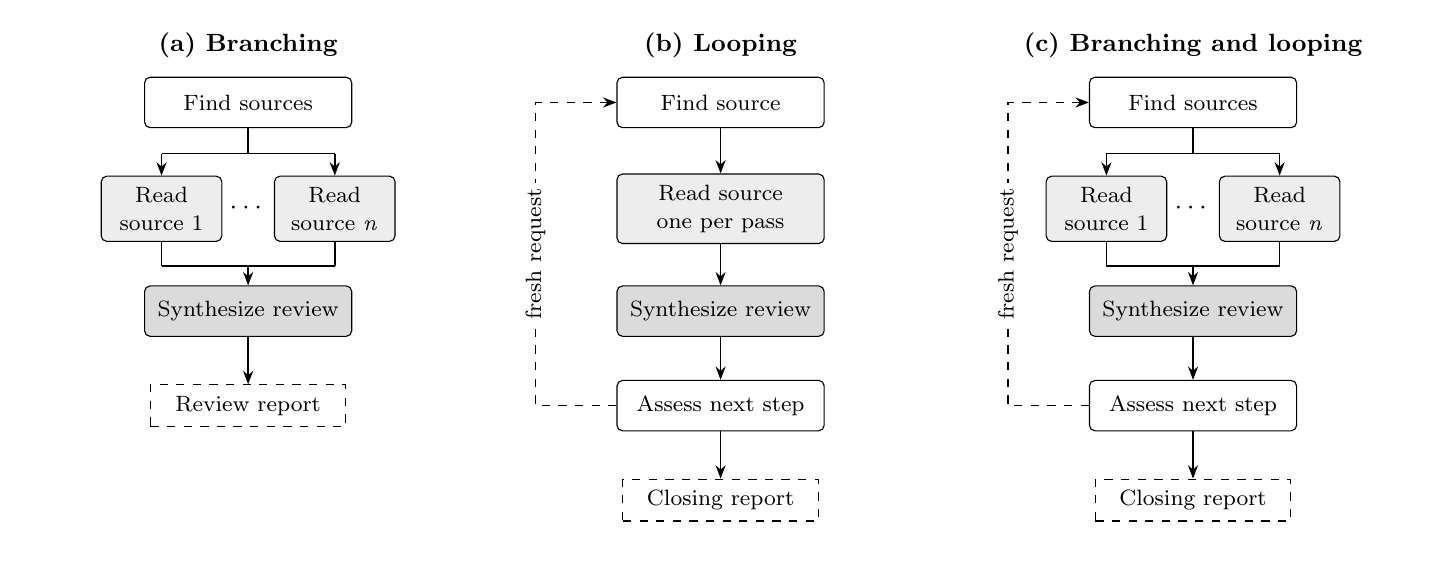
\begin{tikzpicture}[
  operation/.style={draw,rounded corners=2pt,align=center,
    text width=2.35cm,minimum height=.64cm,inner sep=4pt,
    font=\fontsize{8.5}{10}\selectfont},
  reader/.style={operation,fill=black!7},
  synthesis/.style={operation,fill=black!14},
  artifact/.style={draw,dashed,align=center,text width=2.2cm,
    minimum height=.53cm,inner sep=4pt,
    font=\fontsize{8.5}{10}\selectfont},
  handoff/.style={-{Stealth[length=1.7mm]},semithick},
  recurrence/.style={handoff,dashed},
  panel/.style={align=center,text width=5.5cm,inner sep=0pt,
    font=\fontsize{9.5}{11}\selectfont\bfseries},
  annotation/.style={align=center,font=\fontsize{8}{9}\selectfont},
  request/.style={annotation,rotate=90,fill=white,inner sep=2pt}
]
% Explicit bounds make the fragment fit without shrinking its text.
\useasboundingbox (-2.8,-5.48) rectangle (14.97,.95);

\begin{scope}
  \node[panel] at (0,.73) {(a) Branching};
  \node[operation] (a-find) at (0,0) {Find sources};
  \node[reader,text width=1.25cm] (a-read-1) at (-1.1,-1.35) {Read\\source 1};
  \node[reader,text width=1.25cm] (a-read-n) at (1.1,-1.35) {Read\\source \textit{n}};
  \node[font=\normalsize] at (0,-1.35) {$\cdots$};
  \node[synthesis] (a-synth) at (0,-2.65) {Synthesize review};
  \node[artifact] (a-report) at (0,-3.85) {Review report};

  \draw[semithick] (a-find.south) -- (0,-.65);
  \draw[semithick] (-1.1,-.65) -- (1.1,-.65);
  \draw[handoff] (-1.1,-.65) -- (a-read-1.north);
  \draw[handoff] (1.1,-.65) -- (a-read-n.north);
  \draw[semithick] (a-read-1.south) -- (-1.1,-2.08);
  \draw[semithick] (a-read-n.south) -- (1.1,-2.08);
  \draw[semithick] (-1.1,-2.08) -- (1.1,-2.08);
  \draw[handoff] (0,-2.08) -- (a-synth.north);
  \draw[handoff] (a-synth) -- (a-report);
\end{scope}

\begin{scope}[xshift=6cm]
  \node[panel] at (0,.73) {(b) Looping};
  \node[operation] (b-find) at (0,0) {Find source};
  \node[reader] (b-read) at (0,-1.35)
    {Read source\\{\fontsize{8}{9}\selectfont one per pass}};
  \node[synthesis] (b-synth) at (0,-2.65) {Synthesize review};
  \node[operation] (b-assess) at (0,-3.85) {Assess next step};
  \node[artifact] (b-report) at (0,-5.05) {Closing report};

  \draw[handoff] (b-find) -- (b-read);
  \draw[handoff] (b-read) -- (b-synth);
  \draw[handoff] (b-synth) -- (b-assess);
  \draw[handoff] (b-assess) -- (b-report);
  \draw[recurrence] (b-assess.west) -- (-2.35,-3.85)
    -- node[request] {fresh request} (-2.35,0) -- (b-find.west);
\end{scope}

\begin{scope}[xshift=12cm]
  \node[panel] at (0,.73) {(c) Branching and looping};
  \node[operation] (c-find) at (0,0) {Find sources};
  \node[reader,text width=1.25cm] (c-read-1) at (-1.1,-1.35) {Read\\source 1};
  \node[reader,text width=1.25cm] (c-read-n) at (1.1,-1.35) {Read\\source \textit{n}};
  \node[font=\normalsize] at (0,-1.35) {$\cdots$};
  \node[synthesis] (c-synth) at (0,-2.65) {Synthesize review};
  \node[operation] (c-assess) at (0,-3.85) {Assess next step};
  \node[artifact] (c-report) at (0,-5.05) {Closing report};

  \draw[semithick] (c-find.south) -- (0,-.65);
  \draw[semithick] (-1.1,-.65) -- (1.1,-.65);
  \draw[handoff] (-1.1,-.65) -- (c-read-1.north);
  \draw[handoff] (1.1,-.65) -- (c-read-n.north);
  \draw[semithick] (c-read-1.south) -- (-1.1,-2.08);
  \draw[semithick] (c-read-n.south) -- (1.1,-2.08);
  \draw[semithick] (-1.1,-2.08) -- (1.1,-2.08);
  \draw[handoff] (0,-2.08) -- (c-synth.north);
  \draw[handoff] (c-synth) -- (c-assess);
  \draw[handoff] (c-assess) -- (c-report);
  \draw[recurrence] (c-assess.west) -- (-2.35,-3.85)
    -- node[request] {fresh request} (-2.35,0) -- (c-find.west);
\end{scope}
\end{tikzpicture}
\caption{Session patterns specified by three literature-review FAMs. Each
rounded box represents an agent session invoking the named operation. In
(a) and (c), there is one reading session per selected source; the ellipsis
leaves the source count unspecified. These sessions invoke the same
\emph{Read source} schema. Solid arrows show principal artifact dependencies.
Dashed return arrows indicate new passes enabled by fresh requests; dashed
rectangles are output artifacts.}
\label{fig:fam-literature-variants}
\end{figure*}

% Full-page companion to the three literature-review operation patterns.
% Requires tikz with arrows.meta. No scaling: labels are 9--11 pt.
\begin{figure*}[p]
\centering
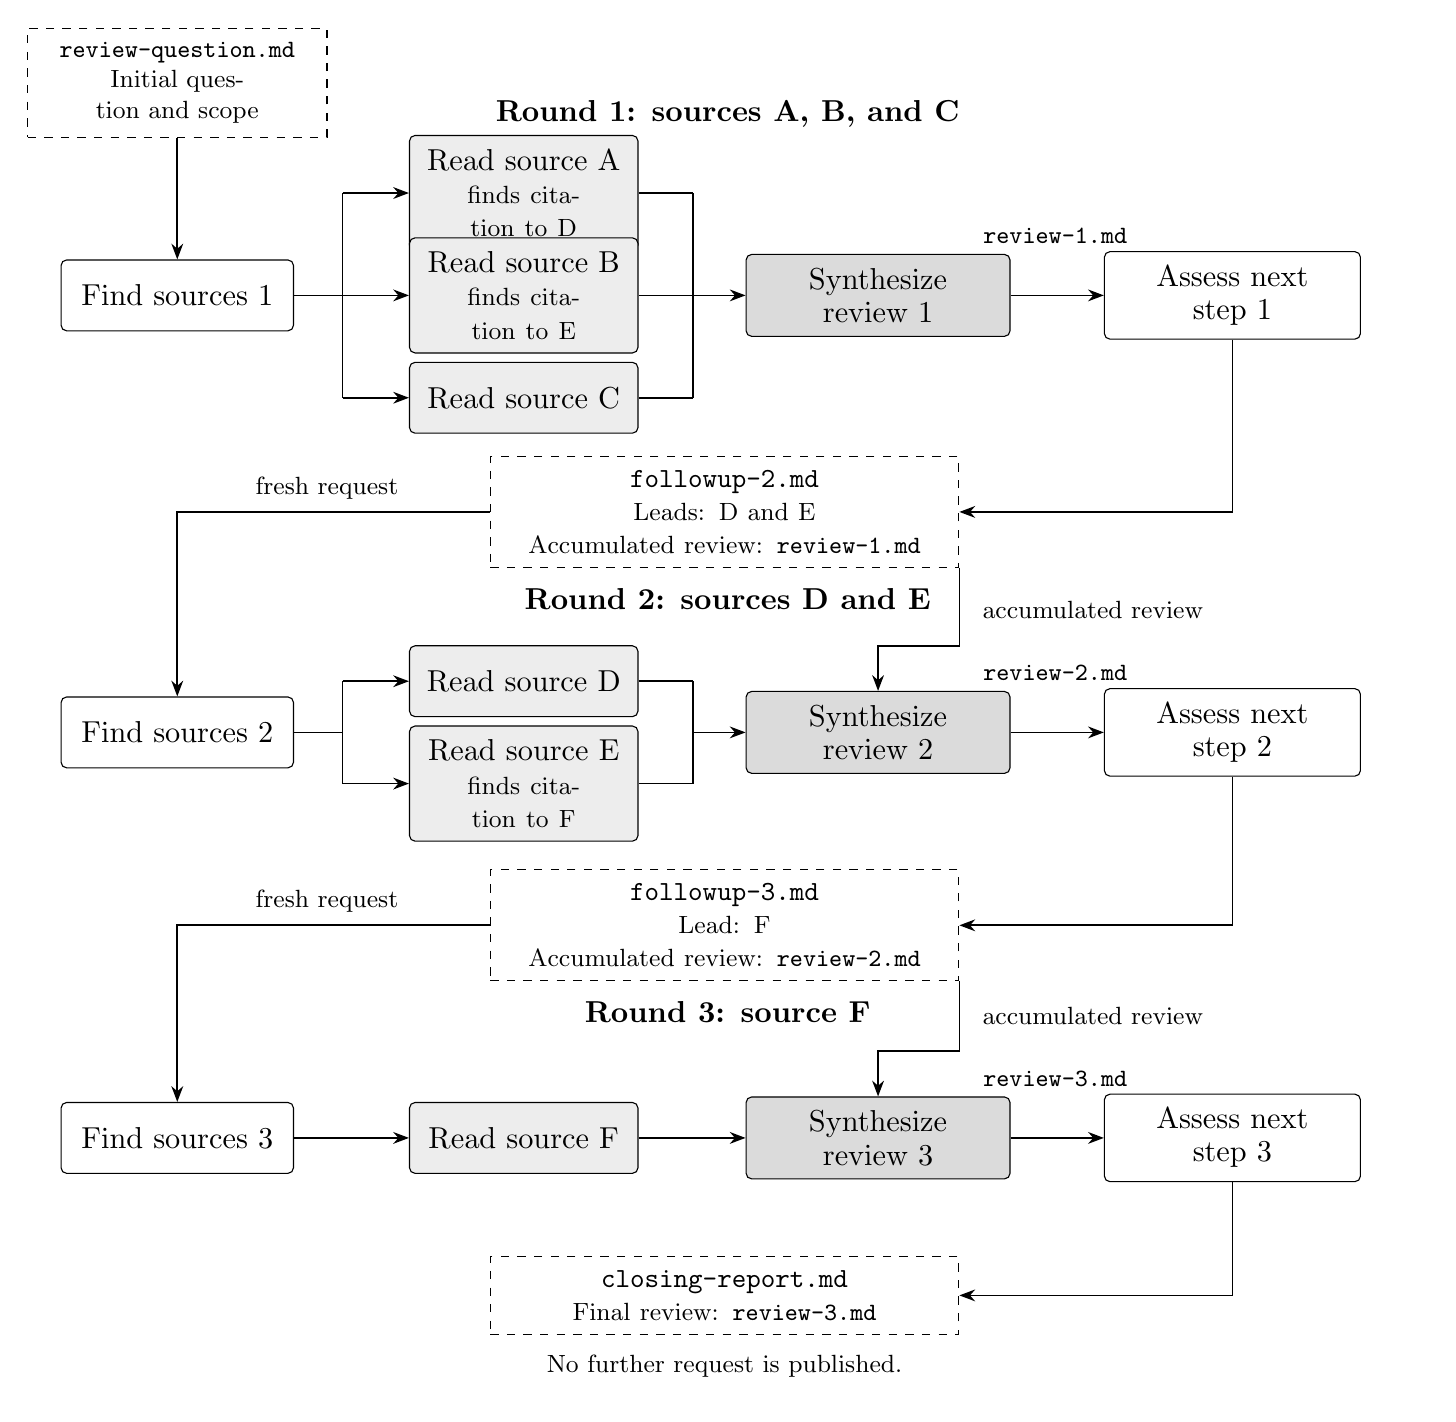
\begin{tikzpicture}[
  execution/.style={draw,rounded corners=2pt,align=center,
    text width=2.6cm,minimum height=.9cm,inner sep=5pt,
    font=\fontsize{10.5}{12}\selectfont},
  reader/.style={execution,fill=black!7,text width=2.55cm},
  synthesis/.style={execution,fill=black!14,text width=3cm},
  assessment/.style={execution,text width=2.9cm},
  artifact/.style={draw,dashed,align=center,text width=5.6cm,
    minimum height=.95cm,inner sep=5pt,
    font=\fontsize{10}{12}\selectfont},
  handoff/.style={-{Stealth[length=2mm]},semithick},
  connector/.style={semithick},
  roundtitle/.style={font=\fontsize{11}{13}\selectfont\bfseries,
    align=center,inner sep=0pt},
  annotation/.style={font=\fontsize{9}{11}\selectfont,
    align=center,fill=white,inner sep=2pt}
]
\useasboundingbox (0,-16.65) rectangle (17.78,.7);

% Initial artifact and the first six completed invocations.
\node[artifact,text width=3.45cm,font=\fontsize{9}{11}\selectfont]
  (question) at (1.9,0)
  {\texttt{review-question.md}\\
   {\fontsize{9}{11}\selectfont Initial question and scope}};
\node[roundtitle] at (8.89,-.4) {Round 1: sources A, B, and C};
\node[execution] (find1) at (1.9,-2.7) {Find sources 1};
\node[reader] (readA) at (6.3,-1.4)
  {Read source A\\{\fontsize{9}{11}\selectfont finds citation to D}};
\node[reader] (readB) at (6.3,-2.7)
  {Read source B\\{\fontsize{9}{11}\selectfont finds citation to E}};
\node[reader] (readC) at (6.3,-4.0) {Read source C};
\node[synthesis] (synth1) at (10.8,-2.7) {Synthesize review 1};
\node[assessment] (assess1) at (15.3,-2.7) {Assess next step 1};
\node[artifact] (followup2) at (8.85,-5.45)
  {\texttt{followup-2.md}\\
   {\fontsize{9}{11}\selectfont Leads: D and E}\\
   {\fontsize{9}{11}\selectfont Accumulated review: \texttt{review-1.md}}};

\draw[handoff] (question) -- (find1);
\draw[connector] (find1.east) -- (4,-2.7);
\draw[connector] (4,-1.4) -- (4,-4.0);
\foreach \source in {A,B,C}{
  \draw[handoff] (4,-2.7 |- read\source.west) -- (read\source.west);
  \draw[connector] (read\source.east) -- (8.45,-2.7 |- read\source.east);
}
\draw[connector] (8.45,-1.4) -- (8.45,-4.0);
\draw[handoff] (8.45,-2.7) -- (synth1.west);
\draw[handoff] (synth1) -- (assess1);
\node[annotation] at (13.05,-1.95) {\texttt{review-1.md}};
\draw[handoff] (assess1.south) -- (15.3,-5.45) -- (followup2.east);

% Five more completed invocations use the same four schemas.
\node[roundtitle] at (8.89,-6.55) {Round 2: sources D and E};
\node[execution] (find2) at (1.9,-8.25) {Find sources 2};
\node[reader] (readD) at (6.3,-7.6) {Read source D};
\node[reader] (readE) at (6.3,-8.9)
  {Read source E\\{\fontsize{9}{11}\selectfont finds citation to F}};
\node[synthesis] (synth2) at (10.8,-8.25) {Synthesize review 2};
\node[assessment] (assess2) at (15.3,-8.25) {Assess next step 2};
\node[artifact] (followup3) at (8.85,-10.7)
  {\texttt{followup-3.md}\\
   {\fontsize{9}{11}\selectfont Lead: F}\\
   {\fontsize{9}{11}\selectfont Accumulated review: \texttt{review-2.md}}};

% The fresh request reaches both source discovery and the next synthesis.
\draw[handoff] (followup2.west) -- (1.9,-5.45) -- (find2.north);
\node[annotation] at (3.8,-5.15) {fresh request};
\draw[handoff] (followup2.south east) |- (10.8,-7.15) -- (synth2.north);
\node[annotation,anchor=west] at (12.05,-6.7) {accumulated review};

\draw[connector] (find2.east) -- (4,-8.25);
\draw[connector] (4,-7.6) -- (4,-8.9);
\foreach \source in {D,E}{
  \draw[handoff] (4,-8.25 |- read\source.west) -- (read\source.west);
  \draw[connector] (read\source.east) -- (8.45,-8.25 |- read\source.east);
}
\draw[connector] (8.45,-7.6) -- (8.45,-8.9);
\draw[handoff] (8.45,-8.25) -- (synth2.west);
\draw[handoff] (synth2) -- (assess2);
\node[annotation] at (13.05,-7.5) {\texttt{review-2.md}};
\draw[handoff] (assess2.south) -- (15.3,-10.7) -- (followup3.east);

% Four final invocations; publication ends without another request.
\node[roundtitle] at (8.89,-11.8) {Round 3: source F};
\node[execution] (find3) at (1.9,-13.4) {Find sources 3};
\node[reader] (readF) at (6.3,-13.4) {Read source F};
\node[synthesis] (synth3) at (10.8,-13.4) {Synthesize review 3};
\node[assessment] (assess3) at (15.3,-13.4) {Assess next step 3};
\node[artifact] (closing) at (8.85,-15.4)
  {\texttt{closing-report.md}\\
   {\fontsize{9}{11}\selectfont Final review: \texttt{review-3.md}}};

\draw[handoff] (followup3.west) -- (1.9,-10.7) -- (find3.north);
\node[annotation] at (3.8,-10.4) {fresh request};
\draw[handoff] (followup3.south east) |- (10.8,-12.3) -- (synth3.north);
\node[annotation,anchor=west] at (12.05,-11.85) {accumulated review};

\draw[handoff] (find3) -- (readF);
\draw[handoff] (readF) -- (synth3);
\draw[handoff] (synth3) -- (assess3);
\node[annotation] at (13.05,-12.65) {\texttt{review-3.md}};
\draw[handoff] (assess3.south) -- (15.3,-15.4) -- (closing.east);
\node[annotation] at (8.85,-16.3) {No further request is published.};
\end{tikzpicture}
\caption{One possible rollout of the branching and looping FAM in
Figure~\ref{fig:fam-literature-variants}(c). Four authored operation schemas
produce 15 completed invocations across three rounds. Each rounded box is
one invocation; dashed boxes identify artifacts. Reading connections
represent the \texttt{request-X.md} and \texttt{assessment-X.md} handoffs for
source X. Fresh requests enable further rounds until a closing report is
published. Arrows show principal artifact dependencies. Intermediate states
are omitted; accumulating output filenames in completion order gives the
state-transition view of Section~\ref{sec:fam-definition-execution}.}
\label{fig:fam-literature-concrete-rollout}
\end{figure*}



\subsection{Branching}

The \emph{Find sources} operation selects relevant sources and publishes a
source-request artifact for each. Each request enables a separate invocation
of \emph{Read source}, which publishes an assessment. \emph{Synthesize review}
combines the assessments into a review. The sources selected during execution
determine which reading branches occur; the same reading schema serves every
selected source.

\subsection{Looping}

The second version examines one source at a time. After \emph{Find source}
and \emph{Read source}, \emph{Synthesize review} incorporates the new assessment
into the accumulated review. \emph{Assess next step} chooses between two
permitted outcomes: a fresh request to investigate a promising citation or
unresolved question, or a closing report. A fresh request enables another
pass through the same operations, with earlier findings carried forward.
The next source and the number of passes are not fixed in advance.

\subsection{Branching and Looping}

The third version repeats the branching process. A round can assess several
selected sources, and synthesis combines their assessments with earlier
findings. \emph{Assess next step} may publish a fresh request for the questions
or citations that warrant more investigation, enabling another round, or a
closing report. Figure~\ref{fig:fam-literature-concrete-rollout} shows one
possible rollout with three sources in the first round, two in the second,
and one in the third before the review concludes.

\section{The Playbook Engine in Alinery}
\label{sec:playbook-engine}

Alinery implements a FAM as a Playbook whose authored steps are instantiated
as executions over particular artifacts. A task retains the selected
Playbook, a shared repository worktree, and the execution history. A session
is the agent process and conversation carrying out an execution. Separating
steps, executions, and sessions allows one reading step to serve many
discovered sources while the engine records which inputs each invocation
received, what it published, and whether its process has stopped.

The filename-set model in Section~\ref{sec:fam-definition-execution} describes
completed agentic transitions. Implementing those transitions requires
additional decisions about input binding, publication, concurrency, and
recovery. Alinery makes those decisions for a local system in which humans
can inspect artifacts and steer ongoing work. Its restrictions on input
modes, workspace access, and recovery are implementation policies rather
than requirements of every FAM.\footnote{The engine and accompanying design
guidance described here are available in the Alinery source at revision
\texttt{054fb36}: \url{https://github.com/DeleganceAI/alinery/tree/054fb36}.}

\subsection{Authored Processes and Agent Judgment}

A Playbook fixes the available step definitions and their dependencies,
while agents determine the concrete work performed within those definitions.
In the literature-review example, an agent chooses which sources merit
reading and whether the accumulated evidence warrants another round. The
engine instantiates the declared reading and continuation steps as the
corresponding artifacts become available. The engine performs no planning
search and does not invent additional collaboration structures. Keeping the
available operations fixed makes the permitted process available for review
before execution, without requiring the author to enumerate the sources,
branches, or number of iterations in advance.

Alinery places domain judgments in agent instructions and artifacts. A
general engine-level condition language would require authors to express
additional decision logic alongside those instructions; the current engine
instead uses declared artifact dependencies to determine readiness. Every
listed input is required, so listing a review and a request creates an AND
dependency. Output declarations describe possible publications, and an
agent can enable different continuations by choosing which outputs to
publish. The engine does not enforce an exclusive choice between two valid
outcomes. If the review procedure requires either a continuation request or
a closing report, the agent instructions must establish that exclusivity.

\subsection{Artifact Identity and Causal Dependencies}

Repeated work requires the engine to distinguish an artifact's logical role
from a particular publication of that role. A logical role such as
\texttt{review.md} identifies a kind of output in the Playbook; an
\emph{artifact occurrence} records one execution's accepted publication,
including its concrete path and producer. Two publications remain distinct
even if they have the same logical role and identical contents. Alinery
assigns separate physical paths to occurrences, while generated depth
numbers and collision suffixes help people navigate the files. Scheduling
uses the recorded occurrences and relationships, independently of those
presentation conventions.

Before starting an execution, the engine binds its inputs to particular
occurrences. Suppose two follow-up requests were derived from different
reviews and the next discovery step requires both a request and its review.
Selecting the most recently written review could give one request evidence
from the other investigation. Alinery uses the recorded relationships
between what executions read and what they published to associate companion
inputs. Missing required inputs leave an execution waiting. When available
inputs leave competing companion pairings unresolved, the engine reports
an ambiguity instead of guessing from timestamps,
zipping files by position, or generating every possible combination.
Authors must supply a dependency structure that makes the intended
relationship recoverable. Once an ordinary input binding has been
scheduled, observing the same binding again does not create duplicate work.

Several steps may publish the same exact logical role, allowing different
routes to enable the same kind of continuation. Each eligible occurrence
retains its own producer and can enable separate work. Wildcard outputs have
a stricter ownership rule: declarations that overlap a wildcard family are
rejected, including an exact output that matches another step's wildcard.
Unique wildcard ownership keeps the attribution of an expanding collection
unambiguous. Sharing an exact role and owning a collection consequently
have different rules, even though both ultimately produce individual
artifact occurrences.

\subsection{Publication, Acceptance, and Process Shutdown}

An artifact file can exist before the engine permits another execution to
consume it. Agents write ordinary files at their assigned paths and then
request completion. The engine checks the requesting execution's ownership
and permission, inspects the assigned outputs, and requires at least one
valid assigned artifact overall. Artifact validation checks for nonempty
regular files at permitted assigned paths; it does not evaluate the claims
in those files or validate their contents against a domain schema.
Additional declared outputs may be
omitted. A source-discovery execution can therefore conclude with a
truthful search report even when it produces no source requests, provided
the report is among its declared outputs. Requiring some accepted evidence
gives successful executions a recorded result without forcing agents to
fabricate a source or continuation merely to fill every output declaration.

Acceptance is atomic across the outputs presented for completion. A present
invalid assigned output rejects the attempt even when another output is
valid, leaving the execution able to repair its files and request completion
again. On acceptance, the engine records the actual publication set in an
immutable receipt. Repeating an accepted completion request returns the same
receipt; files created later cannot enlarge the accepted set. A fixed
receipt makes the result of a lost or repeated completion call inspectable
without interpreting a changing directory as a new publication.

The receipt fixes the publication record, while artifact contents remain
ordinary mutable files. Alinery does not provide immutable byte snapshots
or an operating-system sandbox that intercepts every write. Assigned paths
give agents concrete places to work, and the engine validates publication
against those assignments, but cooperative agents must still respect other
executions' files. Structural acceptance establishes neither the quality of
a source assessment nor compliance with every substantive instruction.
Keeping artifacts directly accessible accommodates existing file-based
tools and human inspection, at the cost of relying on that cooperation for
the integrity of their contents.

Accepted completion also differs from process shutdown. After accepting the
outputs, the engine arranges for the session to finish and waits for
confirmed exit and output drain before launching dependent work. A
completion response therefore acknowledges durable acceptance; it does not
mean that successors have already started. The interval between acceptance
and confirmed shutdown remains visible as finishing work, during which the
session retains its capacity and any coding ownership. Waiting through that
interval prevents the scheduler from treating a still-active producer as
having relinquished its workspace access, although it does not make the
files inaccessible to other tools before exit.

\subsection{Parallel Work and Collection Completeness}

Alinery provides three input modes. A \texttt{single} input binds one exact
artifact occurrence, \texttt{each} creates work for individual collection
members, and \texttt{complete} supplies a completed nonempty collection to
one execution. In the review example, source requests enable separate
reading executions, while synthesis consumes the resulting assessments
together. A step may use at most one collection input, together with any
required exact inputs. Authors who need to relate several collections must
introduce explicit intermediate work rather than relying on an implicit
cross-product join whose intended pairings the engine cannot infer.

Wildcard publication is a batch operation. A producer's files enter the
accepted collection through completion and become available to downstream
work after the producer exits; matching files are not streamed into new
executions as they appear in the directory. Once reading work has been
created, the engine records which contributions are expected. Collection
closure requires those producer and source obligations to be satisfied.
For example, if discovery produced three source requests and only two
readers have finished, two assessment files do not establish that synthesis
is ready. Queued, paused, failed, and finishing work remains accountable.
Waiting for the recorded obligations avoids silently presenting a partial
investigation as the completed collection, while allowing a failed branch
to hold up synthesis until its failure is addressed.

Omitting an intermediate output does not automatically cancel all the work
that would have followed it. Consider two source requests whose readers
may publish triggers for a further extraction step. If one reader publishes
a trigger and the other omits it, the resulting extraction family can remain
incomplete. The engine checks coverage against the relevant members of the
recorded upstream source collection, and no extraction producer represents the source member whose
trigger was omitted. The successful reader has not discharged that downstream
obligation. Where every source needs a downstream disposition, the reader
can instead publish a trigger explaining that a source is unusable, and the
extraction worker can publish a corresponding disposition for synthesis.
The worker and synthesis instructions must define how to handle that outcome.
The engine does not infer branch pruning from missing files or flatten
nested collections into an assumed set of results. Explicit dispositions
require more authoring care, but keep the reason a branch contributes or
stops available in the process itself.

An empty collection also has a specific meaning. A discovery execution may
publish a search summary outside its source-request wildcard and no members
inside the wildcard. Once the relevant obligations close, the collection
is empty: it creates no \texttt{each} workers and does not start an empty
\texttt{complete} consumer. The summary can instead enable an exact handler
or document why the search stopped. A no-result file placed inside the
wildcard is different: it is an ordinary member and enables the corresponding
worker. The engine follows declared membership rather than interpreting
the prose as a signal to suppress execution, so the author must choose
whether a no-result record should itself route work.

\subsection{Iteration, Fresh Evidence, and Stopping}

A loop reuses authored steps through fresh accepted artifact occurrences.
When \emph{Assess next step} publishes another investigation request,
the new request can enable discovery again even though its logical role
has appeared before. Overwriting an earlier request or incrementing a
filename does not by itself create another engine-recognized trigger.
Occurrence-based recurrence distinguishes a new pass from repeated
observation of an existing input binding, allowing the execution history
to grow while the Playbook definition remains fixed.

Freshness also depends on how the author draws the repeated dependencies.
If the next request depends on evaluating a newly synthesized review,
\emph{Assess next step} must consume that review within the repeated
dependency chain. A decision step left dependent on an earlier review can
retain stale evidence even when the Playbook passes syntactic validation.
An unchanged research question may legitimately remain available across
rounds, while an evaluation of changing findings must be renewed. Agents
must also carry
useful accumulated evidence into their handoffs: Alinery records the
execution history but does not automatically summarize that history for
each new session.

The engine imposes no predetermined number of loop passes. The authored
process can continue through fresh publications, produce a stopping report,
or pause for direction. An absence of eligible work establishes only that
the current dependencies enable no further execution; it does not prove
that the investigation answered its question. A closing report can expose
the evidence and reasons for stopping, leaving the human able to distinguish
a supported conclusion from exhaustion, an unresolved dependency, or a need
to revise the investigation. Termination and substantive success remain
separate properties.

\subsection{Shared Workspace and Controlled Concurrency}

Each task has one shared repository worktree. Alinery serializes
engine-managed coding executions within that worktree, avoiding a separate
workspace and subsequent code-merge procedure for every execution.
Independent non-coding investigations can still proceed concurrently.
A coding execution holds exclusive engine-managed access through review,
accepted completion, and confirmed shutdown, because acceptance alone does
not establish that its process has stopped modifying the repository.
The exclusivity rule governs sessions scheduled by the engine; it does not
prevent a user from deliberately editing the repository or starting
auxiliary work.

Coding steps accept exact \texttt{single} inputs. Results from a parallel
investigation must therefore be consolidated into an exact handoff before
they drive coding, giving the coding execution a specific account of the
work to perform. Coding steps may still publish collections for subsequent
non-coding work. Separately, a task-level limit controls the number of live
sessions, with a current default of ten. Additional ready work queues;
starting, waiting-for-human, and finishing sessions continue to occupy
capacity until shutdown or failure to start is confirmed. Capacity and
coding ownership impose different constraints: a free session slot does
not authorize overlapping coding, and a session awaiting human input has
not ceased to be a live process.

\subsection{Human Steering and Explicit Recovery}

Alinery permits useful stretches of automatic progression while retaining
human control over when an execution may finish. When completion requires
human permission, the session stays interactive until the permission is
granted. The grant applies to the particular execution and its owner; the
agent must still finish its work and submit valid outputs for acceptance.
Permission to finish is not approval of immutable artifact bytes, and does
not enable automatic completion for later executions. Keeping permission
separate from acceptance allows a human to review and direct ongoing work
before the agent closes its session.

Failures require explicit recovery. The scheduler does not automatically
retry an execution or transfer its ownership to a replacement session.
An interrupted launch or lost reply may leave uncertainty about whether a
process is still active, so creating another session cannot safely stand in
for establishing what happened to the first. Replacement requires an
explicit ownership transition and evidence that the previous owner stopped.
Recovery can use the existing session and MCP interfaces, including an
external agent acting through MCP, while remaining subject to the same
ownership and permission rules. The cost is that some failures require
attention before work can progress; the engine preserves the unfinished
state instead of selecting a recovery policy on the author's behalf.

Manual publications remain distinct from ordinary graph results. A person
can inspect files, add evidence, or work through an auxiliary session, but
the presence of a matching file does not automatically satisfy an execution's
missing output or discharge an expected worker. Recorded completion must
still attribute the publication to an authorized execution. Keeping manual
work separate preserves the meaning of the graph's execution history while
leaving the task open to human intervention.

\subsection{Durable Execution and Stable Definitions}

The per-repository daemon owns authoritative execution state and scheduling.
The app and MCP act as clients of those operations, while shared core code
implements parsing, validation, and execution rules. Session metadata and
the interface's view of progress are repairable projections of durable
execution records. Centralizing authority in the daemon gives each task's
assignments, permissions, and process lifecycle one governing account,
including when the interface disconnects or restarts.

Alinery persists execution records in local files. Before launching work,
the engine reserves the execution and its output assignments, leaving
inspectable intent if creation or launch fails partway through. A reserved
execution is not proof that its process started; recovery must reconcile
the durable record with the process lifecycle. File-backed persistence
keeps execution state within the local task's storage and backup boundary
without requiring a separate database or distributed execution coordinator.
The implementation must still coordinate reservations and durable writes;
ordinary files do not remove the need to handle partial failure.

A task retains the validated Playbook definition selected at creation.
Later library edits affect future selections, so an investigation does not
silently acquire different instructions or dependencies halfway through a
run. Unknown fields and unsupported syntax are rejected explicitly, keeping
the accepted definition's meaning tied to implemented rules. A missing or
corrupt retained definition is an error rather than permission to substitute
another library version. Current graph execution supports the OMP harness
with configurable model selection. Broader harness support, different
persistence mechanisms, and other resource policies could be implemented
without changing the abstract FAM definition; the behavior described here
is the concrete contract provided by Alinery.

\section{Background}
\label{sec:background}

FAMs bring together two concerns: allowing agents to adapt their work to
discoveries, and making the process that governs that work explicit. Planning,
concurrent-process formalisms, provenance models, and agent frameworks each
provide part of the vocabulary needed to describe that relationship. The
comparisons below distinguish the abstract FAM model from Alinery's concrete
Playbook representation and execution rules. Several existing systems already
support dynamic branching and repetition; the relevant differences concern
how they represent a process, determine eligibility, and record the evidence
behind an execution.

Appendices~\ref{app:claude}--\ref{app:alinery} supply the matched process
definitions for Claude Code, Smithers, LangGraph, and Alinery;
Appendix~\ref{app:shared} supplies their shared prompts, schemas, and fixtures.
The companion document \emph{One Dynamic Literature-Review Process in Four
Agent Systems} (7 October 2026) gives the detailed comparison and verification
scope.\footnote{Appendix listing sources are in \path{whitepaper/examples/}; the companion
document and validation records are linked from \path{whitepaper/BUILD.md}.}
The six-operation process provides a common basis for comparing the four
systems; the motivating examples above isolate branching and looping with
smaller operation sets.

\subsection{Verification Costs and the Scope of Agent Work}

Generating a candidate solution creates another task: determining whether the
candidate is useful and whether its benefits justify the cost of evaluating
it. When an automated evaluator can score each candidate, an agent can search
through alternatives using those scores as feedback. AlphaEvolve combines
language-model-generated program changes with automated evaluation and
evolutionary selection; OpenEvolve provides an open-source implementation of
the same broad approach \cite{novikov2025alphaevolve,sharma2025openevolve}.
The availability and cost of evaluation therefore help determine which
searches are practical. AlphaEvolve explicitly identifies the requirement for
automated evaluation as a limitation of its approach.

Many research and software-development tasks do not come with a complete,
inexpensive evaluator. Tests may establish that a program satisfies particular
examples without establishing that a proposed change addresses the right
problem. A literature review may contain individually accurate summaries while
omitting a relevant line of evidence. In exploratory work, the findings can
also change the question worth pursuing. Producing more candidates can
increase the burden on the people who must assess them, particularly when
mistakes have substantial consequences or the result cannot be conclusively
verified after the work ends.

Task scope and context management provide another reason to organize agent
work into explicit operations. Liu et al. found that the models they studied
often used relevant information less reliably when it appeared in the middle
of a long context, showing that accepting a long input does not ensure
reliable use of its contents \cite{liu2023lostmiddle}. A research operation, an implementation
operation, and a review operation need different instructions and evidence.
Giving each operation a focused responsibility makes its expected inputs and
outputs available for inspection. Practitioner approaches such as
Research--Plan--Implement (RPI) use staged work, context management, and human
review to address the difficulty of carrying a large task through one agent
conversation \cite{dex2025context}. Decomposition still leaves a coordination
problem: someone or something must determine when a subtask is ready, what
evidence it receives, and when its result can be used by others.

An authored process can constrain where effort is spent by requiring evidence
before further investigation, implementation, or review becomes eligible.
Such constraints provide a way to budget verification work and inspect the
path to a result. An execution record can show which activities ran and what
material they used, but following an approved process does not prove the
result correct. Whether process constraints reduce total review effort or
improve outcomes remains an empirical question. FAMs address the coordination
part of that problem by making declared artifact dependencies conditions for
execution, while leaving the substantive assessment of evidence to agents
and people.

\subsection{Reusable Procedures and Agent Coordination}

A process may be generated for one task or retained as a versioned definition
for repeated use. Task-specific generation can be appropriate when the work is
novel and maintaining a reusable procedure would add little value. Retaining
a definition is useful when people want recurring decomposition, review, and
handoff decisions to remain inspectable across executions. The distinction
concerns the lifetime of the process, not its author: a person or an agent may
write either kind of definition. A reusable definition also need not prescribe
a fixed trace; discoveries can determine the number of workers and iterations
within an unchanged set of operations.

Compound Engineering, Compound Writing, and RPI organize agent work through
reusable skills and staged procedures
\cite{everyCompoundEngineering,everyCompoundWriting,dex2025context}.
Prompt-based procedures make expectations explicit and can incorporate human
judgment and review. The coordination requirements expressed in those prompts
still depend on how the agent or surrounding system applies them. A FAM moves
declared input requirements into the execution model: an operation can run
only when an admissible set of inputs is available. That division leaves
agents responsible for interpreting evidence while giving the engine a
separate basis for deciding whether subsequent work is eligible.

Multi-agent frameworks such as AutoGen provide conversation and tool
interaction patterns through which agents can perform and coordinate work
\cite{wu2024autogen}. An agent conversation can also take place within a FAM
operation. The FAM abstraction governs the handoffs between operations,
without specifying every interaction inside them. The distinction matters
for long-running work: an activity may continue across several model or
harness sessions, while downstream operations still need a clear boundary
at which its output becomes available. Prompts, conversations, and execution
rules can therefore serve complementary roles in the same system.

\subsection{Planning Policies and Persistent Execution}

Classical planning supplies precise vocabulary for states, action
applicability, and successor transitions \cite{fikes1971strips}. Hierarchical
task network (HTN) planning supplies authored task decompositions that a
planner refines toward executable networks \cite{erol1994htn}. FAMs use
authored agent operation schemas and input conditions, but the FAM model does
not specify a planner that searches for a sequence or decomposition achieving
a goal. A Playbook fixes the available operation schemas while runtime
artifacts determine which concrete invocations become eligible. The model
therefore concerns execution of an authored process rather than plan
synthesis.

In nondeterministic planning, an action may have more than one possible
result, and a policy associates encountered states with actions so execution
can respond to the result that actually occurs
\cite{kuter2004nondeterministic}. FAMs have a related reactive structure:
an agentic operation can produce different artifacts, and those artifacts
affect which operations can run next. The policy analogy is limited. The FAM
definition supplies a transition relation over artifact states, without a
goal predicate, an optimization objective, or a method for synthesizing a
policy. Alinery further permits several compatible invocations to be eligible
concurrently and records their concrete input bindings and provenance.

The execution horizon is not fixed by the number of authored schemas.
Fresh artifacts can enable additional invocations and potentially
nonterminating rollouts. Planning distinguishes a goal state from a dead end,
where the goal cannot be reached. A FAM supplies no corresponding test for
whether the human's objective has been achieved. At the implementation level,
quiescence means that no work is eligible, queued, or running. Quiescence can
coincide with a useful conclusion or an unproductive stopping point, and later
authorized input may enable more work. A limit on simultaneous sessions
neither establishes eventual termination nor makes the complete state space
finite.

\subsection{Petri Nets and Concurrent Agent Execution}

Petri nets describe processes in which several activities may be enabled at
once and later activities depend on combinations of earlier results. A net
contains \emph{places}, which hold tokens, and \emph{transitions}, which consume
tokens from input places and produce tokens in output places. The distribution
of tokens across all places is the \emph{marking}, or global state of the net.
A transition is enabled when its required input tokens are available;
independent transitions can proceed without imposing an order between them,
while a transition requiring several inputs provides a synchronization point
\cite{jensen1994coloured}.

Colored Petri nets associate typed data values with tokens, allowing a
transition to distinguish particular work items and match their associated
inputs \cite{jensen1994coloured}. Read arcs add a complementary operation:
requiring a token to be present without consuming it
\cite{rodriguez2012readarcs}. Reusable information can therefore enable several
activities, while ordinary consuming arcs can represent resources whose use
must be exclusive.

Playbooks implement an artifact-driven concurrent execution model closely
related to colored Petri nets with read arcs. A Playbook defines agentic
operations called Steps and connects them through declared artifact inputs and
possible outputs. Each execution binds a Step to particular artifact
occurrences, retaining the identity of each publication and its producing
execution. In a Petri-net interpretation, occurrences provide data-bearing
tokens, input requirements determine enabling conditions, and accepted
publications supply new tokens. For example, two reviewers may read the same
brief independently, while a synthesis Step requires both review results.
Read arcs express reuse of the brief, and the synthesis inputs express the
AND dependency. Occurrence and provenance information distinguishes results
from different requests or loop passes.

The engine also records behavior that a faithful net model would need to make
explicit. An execution occupies capacity while active, and its accepted
outputs become available to dependent executions only after shutdown is
confirmed. Recorded input bindings prevent duplicate automatic executions;
session limits and exclusive coding access constrain launches. Collection
inputs support one execution per member and synchronization over a nonempty
accepted collection after all expected contributors and source obligations
have completed. Agent outcomes introduce nondeterminism in artifact contents
and in the permitted outputs published. Publication of the required artifact
roles determines downstream eligibility; agents interpret artifact contents.

The Petri-net comparison identifies a structural relationship rather than an
established formal equivalence. An exact encoding would need to preserve
occurrence matching, binding deduplication, collection closure, and execution
lifecycle rules. A finite set of Step definitions can generate an unbounded
number of executions and artifact occurrences, just as a finite net description
does not by itself bound the number of reachable markings. The abstract FAM
definition captures artifact availability; the additional lifecycle and
provenance rules belong to Alinery's implementation.

\subsection{Workflow Languages and Statecharts}

Workflow languages commonly represent splits, joins, choices, and loops as
control-flow patterns \cite{vanderAalst2003workflow}; statecharts likewise make
control state and transitions explicit \cite{harel1987statecharts}. A Playbook
can be rendered with similar shapes. Its eligibility rules, however, are
expressed through artifact requirements, and Alinery resolves those
requirements using occurrence identity and provenance. An operation's position
in the authored document is not a cursor that determines what happens next.

The distinction between a process definition and its execution record is
particularly useful for loops. A definition may contain a visual cycle because
an operation can become eligible again, while successive invocations and their
publications extend a forward causal history. FAMs use artifact availability
to describe that continuation. Workflow and statechart formalisms already
provide ways to express recurrence; the FAM choice centers the handoff
artifacts and, in Alinery, the recorded reason that each invocation occurred.

\subsection{Temporal Execution and Provenance}

Temporal planning for actions with duration distinguishes an action's interval
of execution from the points at which its effects change the state
\cite{fox2003pddl21}. Agent execution requires a related distinction between
work in progress and outputs available to dependent work. In Alinery, a Step
execution can span sequential harness sessions, while output acceptance and
confirmed producer exit establish the downstream handoff boundary. The
analogy does not import the temporal constraints, time-varying numeric state
variables, or formal plan validation of the Planning Domain Definition
Language (PDDL).

General provenance models describe entities, activities, agents, and
derivations \cite{moreau2013prov}. Alinery specializes that vocabulary by
recording artifact occurrences, their producing executions, and the exact
bindings used by subsequent executions. Two publications remain distinct
events even when their logical names or contents match. Those identities let
the engine associate assessments with the requests that generated them and
distinguish one loop pass from another. The abstract FAM state is only the set
of available filenames; execution provenance supplies additional information
about how the state was reached.

Provenance establishes a record of the handoff, not the truth of an artifact's
contents. Alinery's accepted publication records do not make the underlying
files immutable or create a security sandbox. Likewise, a complete collection
of assessments establishes that the expected contributors supplied their
outputs, not that their conclusions are sound. Keeping structural completion
separate from substantive validation makes the engine's guarantees and the
remaining responsibilities of agents and reviewers explicit.

\subsection{Claude Code Dynamic Workflows}

Claude Code Dynamic Workflows express agent coordination as a JavaScript
script executed by a runtime outside the supervising conversation. The script
invokes agents, retains intermediate results in variables, and uses ordinary
conditions and loops to determine subsequent work. Operations such as
\texttt{pipeline} dispatch an agent for each item in a list, allowing the number
of workers to depend on discoveries made during execution. In the matched
literature-review example, the script discovers sources, launches a reader for
each source, waits for the assessments, and repeats discovery when the decision
agent requests another round. A saved script therefore defines a reusable
process whose concrete execution can vary without changing its orchestration
code \cite{anthropic2026dynamicworkflows}.

The principal difference from FAMs concerns how the process represents
dependencies and continuation. A Claude workflow expresses ordering through
program execution: the script awaits results, evaluates conditions, and invokes
the next operation. A FAM expresses eligibility through the availability of
declared input artifacts, with published outputs enabling subsequent
operations. In Alinery, a Playbook places agent instructions alongside artifact
declarations, and the engine binds each execution to particular artifact
occurrences. Reviewing the coordination rules therefore centers on the
declared handoffs, while reviewing a Claude workflow centers on its JavaScript
control flow. The enforcement boundaries also differ: Claude supports
structured agent responses that the script can inspect, whereas the FAM
abstraction leaves artifact contents opaque and assigns their interpretation
to agents.

\subsection{Smithers}

Smithers organizes execution through typed actions and flows. A flow body
constructs a plan for one round, describing action dependencies, concurrent
work, and conditional branches before the round executes. Runtime discoveries
can determine the shape of a later round: the current round hands its results
to another flow, whose body constructs a plan from the received payload. In
the matched literature-review example, discovery supplies the source list to
a reader round, which creates one action per source and combines their results
through \texttt{Node.all}. A later decision either completes the process or
hands control back to discovery. The authored flows remain fixed while the
number of readers and rounds varies with the evidence
\cite{smithers2026plans,smithers2026rounds}.

Smithers and FAMs both make dependencies explicit, but organize dynamic
execution around different objects. Smithers constructs a round's plan from
a typed payload and represents continuation through an explicit handoff to
another flow. A FAM repeatedly applies reusable operation schemas as their
artifact requirements become satisfied. In Alinery, publishing source-request
artifacts enables individual reader executions; collection requirements
determine when their assessments can enable synthesis; and a new continuation
artifact enables another discovery execution. The reader population therefore
follows artifact publication and binding rules, without the Playbook author
constructing a separate plan for each round. Smithers also gives payload and
result schemas a central role, while FAM input and output specifications
describe artifact availability and leave content interpretation outside the
abstract coordination model.

\subsection{LangGraph}

LangGraph represents an agent application as a graph whose nodes perform
operations over application state. Nodes return state updates, reducers
determine how updates are combined, and edges or routing functions determine
which nodes execute next. LangGraph supports work whose size becomes known
only during execution: a routing function can return one \texttt{Send} per
discovered item, each carrying inputs for a separate node invocation. In the
matched literature-review example, discovery dispatches a reader for each
fresh source, the runtime coordinates the reader batch before synthesis, and
conditional routing either returns to discovery or terminates. The graph
defines reusable operations while intermediate results determine their
invocation count and execution path
\cite{langchain2026graphapi,langchain2026pregel}.

The major difference from FAMs lies in the representation of state and the
rules that connect successive operations. LangGraph provides
application-defined state fields, update functions, and routing logic; the
FAM abstraction represents state as a set of available artifact filenames,
extended by publication while previously available filenames remain present.
Alinery adds concrete occurrence identities and execution provenance,
recording which publications supplied an operation's inputs even when logical
artifact names recur across iterations. For the literature-review process,
the LangGraph implementation explicitly manages round identifiers and
accumulated assessments, while the Playbook declares the artifact
relationships used to select and join the corresponding work. The distinction
is a choice of coordination model and authoring interface; dynamic branching,
synchronization, and repetition are capabilities shared by both approaches.

\subsection{Scope of the Comparison}

The matched examples use the same intended literature-review process:
frame a question, discover fresh sources, read each source, combine the
current batch with prior evidence, and decide whether to continue. Empty
discovery has a separate terminal route. The examples compare where those
decisions and dependencies are represented. They do not establish identical
behavior for every malformed response: the programmatic examples include
response guards, while the Alinery example leaves semantic conditions such as
source identity and exclusive publication of a continuation or stopping
artifact in the agent instructions. The comparison also does not establish
that a Playbook is easier to review, that the representation is architecturally
novel, or that any system produces better research. Fixture checks exercise
selected orchestration behavior; the Claude example was checked through a
compatibility harness, and no live-model comparison was performed.

Appendix~\ref{app:playbook-definition} retains a complementary
research-to-design example: Frame derives research questions, Discover
identifies sources, Appraise evaluates question--source pairs, Synthesize
combines the appraisals for each question, and Design integrates the findings
and may request follow-up research. Its keyed collections and
\texttt{fulfills} relationships associate requests with results, while
\texttt{complete-set} and \texttt{when} express the intended merge conditions.
The listing is preserved schematic notation, not the current supported
Playbook serialization. Section~\ref{sec:playbook-engine} explains the
implemented coordination rules and their design tradeoffs. Neither a schematic example nor an
execution trace establishes general correctness, scalability, termination
under failure, operational security, or the quality of agent outputs.


{\small
\bibliography{references}
}

\clearpage
\appendix
\section{Schematic Playbook Definition}
\label{app:playbook-definition}

Listing~\ref{lst:playbook} records a compact definition of the running example.
The notation names the semantic relationships used in the paper without
freezing a portable serialization format. Agent instructions, harness
selection, resource policy, and output paths remain part of a complete Step
definition even where the schematic elides them.

\begin{listing}[H]
\begin{lstlisting}
playbook: research-to-design
collections:
  appraisal-requests: key(question, source)
  appraisal-results: fulfills(appraisal-requests)
  question-synthesis-requests: key(question)
  question-syntheses: fulfills(question-synthesis-requests)
  followup-research: key(handoff)
  framed-questions: fulfills(followup-research)
  design-requests: key(design)

steps:
  frame:
    input: each(followup-research)
    output: framed-questions
  discover:
    input: each(framed-questions)
    emit: [appraisal-requests,
           question-synthesis-requests,
           design-requests]
  appraise:
    input: each(appraisal-requests)
    output: appraisal-results
  synthesize:
    input: each(question-synthesis-requests)
    complete-set: required-appraisals(input)
    when: all-appraisals-from-expansion-fulfilled
    output: question-syntheses
  design:
    input: each(design-requests)
    complete-set: required-syntheses(input)
    output: [design.md, followup-research]
\end{lstlisting}
\caption{Schematic research-to-design Playbook. An initial agenda is represented
as the first member of \texttt{followup-research}; later Design executions may
emit another member or an explicitly empty collection.}
\label{lst:playbook}
\end{listing}

\clearpage
\onecolumn
\lstset{style=comparison-source}
\section*{Matched Literature-Review Implementations}
The following appendices contain the four complete implementation examples
and their shared prompts, schemas, and fixture data. All displayed file paths
are relative to \path{whitepaper/examples/}; preserve the sibling
\file{claude/}, \file{smithers/}, \file{langgraph/}, \file{alinery/}, and
\file{shared/} directories. The files printed here are included directly
from that directory.

The full \emph{source bundle}, linked from \path{whitepaper/BUILD.md},
additionally contains test drivers, dependency lockfiles, generators, and
captured evidence. Reproduction commands below assume that full bundle.

Claude's appendix prints the process body and generator, which produces the
self-contained workflow script. The Alinery appendix prints the complete
generated Playbook. Smithers and LangGraph include their live entry points
and authored helpers. The examples retain their original verification
boundaries and do not claim live-model validation.

\section{Claude Code Dynamic Workflow}\label{app:claude}
Save the following files under \file{claude/}, alongside the \file{shared/} directory in Appendix~\ref{app:shared}. Build with Node 22 or later (26.0.0 was used). No npm dependencies are needed. The body intentionally uses the native workflow environment's top-level \texttt{return}; execute its generated file through Claude Code, not as an ordinary Node program. The \texttt{agent} and \texttt{pipeline} functions and \texttt{args} global are provided by Claude's native runtime.\cite{anthropic2026dynamicworkflows}
\begin{lstlisting}
cd claude
npm run build
mkdir -p .claude/workflows
cp matched-literature-review.js .claude/workflows/matched-literature-review.js
claude
\end{lstlisting}
After authenticating separately, enter the following at Claude's interactive prompt. If the session was already open, run \texttt{/reload-skills} first. Native execution remains unverified in this draft.
\begin{lstlisting}
Run /matched-literature-review with args {"question":"How can agent execution follow a reusable process while adapting the number of workers and iterations to discoveries?"}. Execute the saved script unchanged.
\end{lstlisting}
\sourcefile{Native process body}{claude/workflow.body.js}
\sourcefile{Self-contained script generator}{claude/build.mjs}
\sourcefile{Build manifest}{claude/package.json}
The bundle's \file{claude/test.mjs} and \file{claude/checks.json} document compatibility verification. Run \texttt{npm test} to reproduce it. The generated \file{claude/matched-literature-review.js} embeds the exact shared constants followed by the body above.

\clearpage
\section{Smithers flow}\label{app:smithers}
Use the exact Smithers source revision below. \file{register.mjs} maps unpublished package exports to unmodified upstream source and checks the commit. The supplied \file{package-lock.json} pins the npm dependency tree. From the \file{smithers/} directory:
\begin{lstlisting}
git clone https://github.com/smithersai/smithers.git ../smithers-source
git -C ../smithers-source checkout 8fee1a6d88ef0308159cb1c9bd6a462ebf660724
npm ci --no-audit --no-fund
npm test
npm run live -- 'Your research question'
\end{lstlisting}
The final command requires an authenticated Claude CLI and performs live inference. An existing source checkout can instead be supplied with \texttt{SMITHERS\_SOURCE}. The fixture checks use the actual native engine; the live adapter is unverified. CLI structured-output flags follow the installed help and official reference.\cite{anthropic2026clireference}
\sourcefile{Process and native engine wiring}{smithers/process.mjs}
\sourcefile{Agent I/O and output guards}{smithers/agents.mjs}
\sourcefile{Upstream source resolver}{smithers/register.mjs}
\sourcefile{Live entry point}{smithers/run.mjs}
\sourcefile{Dependency manifest}{smithers/package.json}
The bundle includes \file{smithers/test.mjs}, \file{smithers/test-report.json}, and the exact npm lockfile. The in-memory runtime is sufficient for this example; no stable cross-process callback identity or durable restart is claimed.

\clearpage
\section{LangGraph graph}\label{app:langgraph}
From \file{langgraph/}, install the pinned dependencies and run the native fixture checks. Use Python 3.14.5 to reproduce the checked environment.
\begin{lstlisting}
python3 -m venv .venv
.venv/bin/python -m pip install -r requirements.lock
.venv/bin/python verify.py
.venv/bin/python run.py --mode fixture --scenario normal --output run.json
.venv/bin/python run.py --mode live --question-file ../shared/question.txt --output live-run.json
\end{lstlisting}
The final command requires authenticated Claude Code. Its output file records the report and execution evidence. The default concurrency is eight; the default super-step safety limit is 1000. Neither fixes the scientific number of readers or rounds. No durable checkpointer is configured.
\sourcefile{Process graph}{langgraph/process.py}
\sourcefile{Agent I/O adapters}{langgraph/agents.py}
\sourcefile{Entry point and native run evidence}{langgraph/run.py}
Native checks and per-scenario traces are supplied in \file{langgraph/verify.py} and \file{langgraph/evidence/}. Fixture outputs do not validate the live adapter or the quality of a literature review.
\sourcefile{Complete dependency lock}{langgraph/requirements.lock}

\clearpage
\section{Alinery Playbook (FAM)}\label{app:alinery}
This is the complete v2 Playbook for Alinery source snapshot \file{d9768d9a8dbea228860e2a4408f7079a5952e788} (core version 0.20.1). Copy it into the target research repository's Playbook library, preserving the filename:
\begin{lstlisting}
review_repo=/absolute/path/to/research-repository
mkdir -p "$review_repo/.alinery/playbooks/matched-literature-review"
cp alinery/playbook.md "$review_repo/.alinery/playbooks/matched-literature-review/playbook.md"
\end{lstlisting}
Choose \emph{Matched Literature Review} when creating a task in that repository; use the common question as its description. Select an authenticated OMP configuration with web research tools, automatic advancement for all six steps, and capacity for at least two sessions. Respect existing completion locks. These are live-use instructions; no desktop app or live harness was launched during verification.

The \texttt{frame} step has no graph input and reads the original ticket once. The loop starts with its round request. Logical output names are roles, not physical filenames: agents must use the engine's assigned paths and provenance-bound input lists. Empty discovery publishes an explicit disposition because a missing collection is not a completed empty batch. A branch selects outputs through the agent's publication behavior; output declarations are not an exclusive-or constraint.
\sourcefile{Complete Playbook definition}{alinery/playbook.md}
The bundle contains \file{alinery/build_playbook.py}, which reproduces this file from the shared prompts and file mappings. Live execution needs only the generated Playbook. The native core checks use \file{alinery/verify.py} and \file{alinery/verify.rs}:
\begin{lstlisting}
python3 alinery/verify.py --alinery-source /absolute/path/to/alinery
\end{lstlisting}
Cargo dependencies must already be cached because this verifier runs offline. It constructs a temporary test project against production \texttt{alinery-core}; it does not replace the scheduler, edit product code, or launch a daemon. Its record is \file{validation/alinery.json}.

\clearpage
\section{Shared prompts, schemas, and fixture data}\label{app:shared}
These files specify the common process contract. Prompts define the operation's domain work; schemas specify its response shape. Claude, Smithers and LangGraph consume these schemas directly; the Alinery Playbook uses textual field descriptions and the shared domain instructions. The schema alone does not encode every cross-field condition, so the examples also contain the guards or prompt obligations described earlier. Preserve these files in \file{shared/}, as a sibling of the four implementation directories.

\sourcefile{Default research question}{shared/question.txt}
\sourcefile{Canonical operation prompts}{shared/prompts.json}
\sourcefile{Complete JSON response schemas}{shared/schemas.json}
\sourcefile{Synthetic fixture responses}{shared/fixtures.json}

The fixture URLs are intentionally invalid. They exercise orchestration without network access or paid model calls. A live run uses actual discovered sources; it must never present fixture text as a literature finding. The source bundle includes all test drivers and the captured verification outputs; their exact scope is described in each implementation's \file{RUNNING.md}.
\end{document}
